\section{Mesh Router}

\begin{frame}{Anwendungsbeispiele}
    \begin{block}{Anschlüsse}
        \begin{itemize}
            \item Client-Ports \& Infrastructure Funknetz:
                Wie ein großer Switch
            \item Batman-Ports \& Ad-Hoc Funknetz:
                Mesh-Netz
            \item WAN-Ports:
                VPN Netz
        \end{itemize}
        \center{
            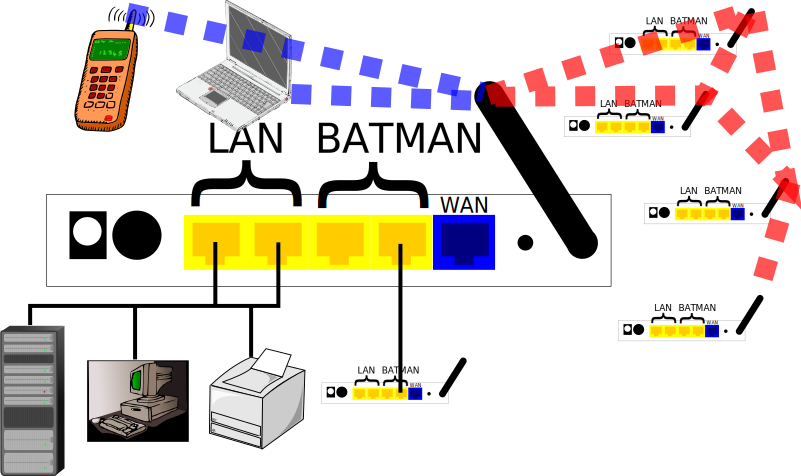
\includegraphics[width=0.75\textwidth]{img/svg/anschluesse.pdf}
        }
    \end{block}
\end{frame}

\begin{frame}{Anwendungsbeispiele}
    \begin{block}{Autarkes Layer-2 Netz}
        Eine Wolke kann ihr Netz von einem Router bekommen der an einen der
        Client-Ports angeschlossen wird.

        \center{
            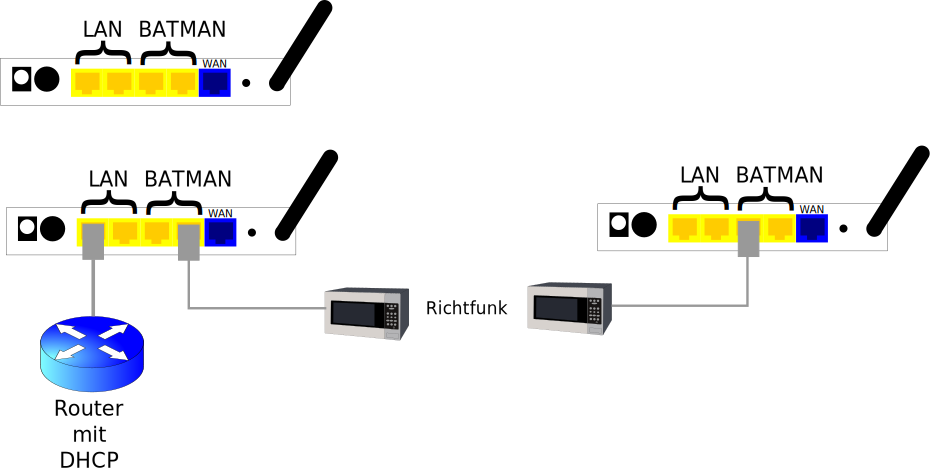
\includegraphics[width=0.8\textwidth]{img/svg/als_grosses_wlan.pdf}
        }
    \end{block}
\end{frame}

\begin{frame}{Anwendungsbeispiele}
    \begin{block}{Standort mit mehreren Kanälen}
        Mehrere Knoten können beliebig untereinander per Kabel verbunden werden.

        \center{
            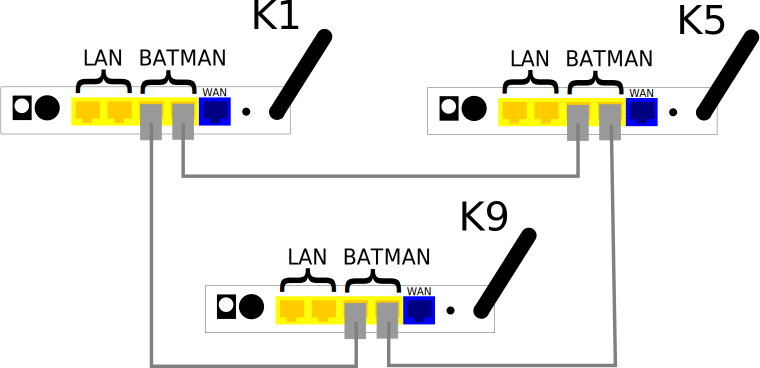
\includegraphics[width=0.9\textwidth]{img/svg/knoten_mit_mehr_kanaelen_richtungen.pdf}
        }
    \end{block}
\end{frame}


\begin{frame}{Mesh Router}
%Danach geht der Vortrag auf den inneren Aufbau der Router Software
%(Firmware) ein. Es wird gezeigt, welche Aufgabe ein Router konkret
%zu erfüllen hat.

\begin{block}{
    \only<1-2>{Jeder Knoten ist wie ein großer Switch}
    \only<3-4>{Das Freifunk-Netz besteht aus}
}

\renewcommand{\arraystretch}{1.5}
\begin{tabular}{|c|c|c|c|c|c|c|} \hline
 \multicolumn{7}{|c|}{\alt<3-4>{\textcolor{gray}{Bridge}}{Bridge}} \\ \hline
 \multirow{2}{*}{\alt<3-4>{\textcolor{gray}{Managed}}{Managed}} &
 \multicolumn{4}{c|}{\visible<2->{B.A.T.M.A.N}} &
 \multicolumn{2}{c|}{\multirow{2}{*}{\alt<3-4>{\textcolor{gray}{Client-VLan}}{Client-VLan}}} \\ \cline{2-5}
 & \visible<3->{Ad-Hoc} & \visible<4->{VPN} & \multicolumn{2}{c|}{\visible<3->{Node-VLan}} & \multicolumn{2}{c|}{} \\ \hline
 \multicolumn{2}{|c|}{Wifi} & \visible<4->{WAN} & \visible<3->{LAN1} & \visible<3->{LAN2} &
 \alt<3-4>{\textcolor{gray}{LAN3}}{LAN3} & \alt<3-4>{\textcolor{gray}{LAN4}}{LAN4} \\ \hline
\end{tabular}

\only<1-2>{
        \begin{itemize}
            \item Clients, die sich vor Ort per WLan verbinden
            \item Clients, die sich per Kabel verbinden
            \item<2> Das Freifunk-Netz
        \end{itemize}
}
\only<3-4>{
    \begin{itemize}
        \item Knoten, die sich über WLan verbinden
        \item Knoten, die sich über Kabel verbinden
        \item<4> Knoten, die über VPN verbunden werden
    \end{itemize}
}

\end{block}

\end{frame}


%\begin{frame}{Wifi - Ad-Hoc}
%    % TODO MAC Adressen ???
%\renewcommand{\arraystretch}{1.5}
%\begin{tabular}{|c|c|c|c|c|c|c|} \hline
% \multicolumn{7}{|c|}{Bridge :01} \\ \hline
% \multirow{2}{*}{Managed :01} & \multicolumn{4}{c|}{B.A.T.M.A.N :rr} & \multicolumn{2}{c|}{\multirow{2}{*}{Client-VLan :02}} \\ \cline{2-5}
% & Ad-Hoc :01 & VPN :rr & \multicolumn{2}{c|}{Node-VLan :02} & \multicolumn{2}{c|}{} \\ \hline
% \multicolumn{2}{|c|}{Wifi :01} & WAN :02 & LAN1 :02 & LAN2 :02 & LAN3 :02 & LAN4 :02 \\ \hline
%\end{tabular}
%
%\end{frame}

